\documentclass[1p]{elsarticle_modified}
%\bibliographystyle{elsarticle-num}

%\usepackage[colorlinks]{hyperref}
%\usepackage{abbrmath_seonhwa} %\Abb, \Ascr, \Acal ,\Abf, \Afrak
\usepackage{amsfonts}
\usepackage{amssymb}
\usepackage{amsmath}
\usepackage{amsthm}
\usepackage{scalefnt}
\usepackage{amsbsy}
\usepackage{kotex}
\usepackage{caption}
\usepackage{subfig}
\usepackage{color}
\usepackage{graphicx}
\usepackage{xcolor} %% white, black, red, green, blue, cyan, magenta, yellow
\usepackage{float}
\usepackage{setspace}
\usepackage{hyperref}

\usepackage{tikz}
\usetikzlibrary{arrows}

\usepackage{multirow}
\usepackage{array} % fixed length table
\usepackage{hhline}

%%%%%%%%%%%%%%%%%%%%%
\makeatletter
\renewcommand*\env@matrix[1][\arraystretch]{%
	\edef\arraystretch{#1}%
	\hskip -\arraycolsep
	\let\@ifnextchar\new@ifnextchar
	\array{*\c@MaxMatrixCols c}}
\makeatother %https://tex.stackexchange.com/questions/14071/how-can-i-increase-the-line-spacing-in-a-matrix
%%%%%%%%%%%%%%%

\usepackage[normalem]{ulem}

\newcommand{\msout}[1]{\ifmmode\text{\sout{\ensuremath{#1}}}\else\sout{#1}\fi}
%SOURCE: \msout is \stkout macro in https://tex.stackexchange.com/questions/20609/strikeout-in-math-mode

\newcommand{\cancel}[1]{
	\ifmmode
	{\color{red}\msout{#1}}
	\else
	{\color{red}\sout{#1}}
	\fi
}

\newcommand{\add}[1]{
	{\color{blue}\uwave{#1}}
}

\newcommand{\replace}[2]{
	\ifmmode
	{\color{red}\msout{#1}}{\color{blue}\uwave{#2}}
	\else
	{\color{red}\sout{#1}}{\color{blue}\uwave{#2}}
	\fi
}

\newcommand{\Sol}{\mathcal{S}} %segment
\newcommand{\D}{D} %diagram
\newcommand{\A}{\mathcal{A}} %arc


%%%%%%%%%%%%%%%%%%%%%%%%%%%%%5 test

\def\sl{\operatorname{\textup{SL}}(2,\Cbb)}
\def\psl{\operatorname{\textup{PSL}}(2,\Cbb)}
\def\quan{\mkern 1mu \triangleright \mkern 1mu}

\theoremstyle{definition}
\newtheorem{thm}{Theorem}[section]
\newtheorem{prop}[thm]{Proposition}
\newtheorem{lem}[thm]{Lemma}
\newtheorem{ques}[thm]{Question}
\newtheorem{cor}[thm]{Corollary}
\newtheorem{defn}[thm]{Definition}
\newtheorem{exam}[thm]{Example}
\newtheorem{rmk}[thm]{Remark}
\newtheorem{alg}[thm]{Algorithm}

\newcommand{\I}{\sqrt{-1}}
\begin{document}

%\begin{frontmatter}
%
%\title{Boundary parabolic representations of knots up to 8 crossings}
%
%%% Group authors per affiliation:
%\author{Yunhi Cho} 
%\address{Department of Mathematics, University of Seoul, Seoul, Korea}
%\ead{yhcho@uos.ac.kr}
%
%
%\author{Seonhwa Kim} %\fnref{s_kim}}
%\address{Center for Geometry and Physics, Institute for Basic Science, Pohang, 37673, Korea}
%\ead{ryeona17@ibs.re.kr}
%
%\author{Hyuk Kim}
%\address{Department of Mathematical Sciences, Seoul National University, Seoul 08826, Korea}
%\ead{hyukkim@snu.ac.kr}
%
%\author{Seokbeom Yoon}
%\address{Department of Mathematical Sciences, Seoul National University, Seoul, 08826,  Korea}
%\ead{sbyoon15@snu.ac.kr}
%
%\begin{abstract}
%We find all boundary parabolic representation of knots up to 8 crossings.
%
%\end{abstract}
%\begin{keyword}
%    \MSC[2010] 57M25 
%\end{keyword}
%
%\end{frontmatter}

%\linenumbers
%\tableofcontents
%
\newcommand\colored[1]{\textcolor{white}{\rule[-0.35ex]{0.8em}{1.4ex}}\kern-0.8em\color{red} #1}%
%\newcommand\colored[1]{\textcolor{white}{ #1}\kern-2.17ex	\textcolor{white}{ #1}\kern-1.81ex	\textcolor{white}{ #1}\kern-2.15ex\color{red}#1	}

{\Large $\underline{11a_{7}~(K11a_{7})}$}

\setlength{\tabcolsep}{10pt}
\renewcommand{\arraystretch}{1.6}
\vspace{1cm}\begin{tabular}{m{100pt}>{\centering\arraybackslash}m{274pt}}
\multirow{5}{120pt}{
	\centering
	\includegraphics[width=112pt]{../../../GIT/diagram.site/Diagrams/png/256_11a_7.png}\\
\ \ \ A knot diagram\footnotemark}&
\allowdisplaybreaks
\textbf{Linearized knot diagam} \\
\cline{2-2}
 &
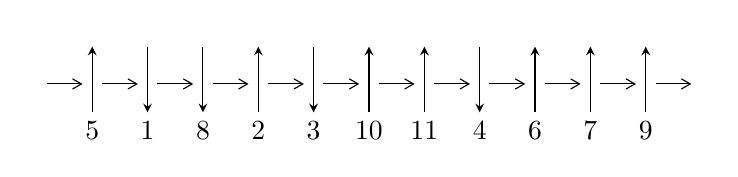
\begin{tikzpicture}[x=20pt, y=17pt]
	% nodes
	\node (C0) at (0, 0) {};
	\node (C1) at (1, 0) {};
	\node (C1U) at (1, +1) {};
	\node (C1D) at (1, -1) {5};

	\node (C2) at (2, 0) {};
	\node (C2U) at (2, +1) {};
	\node (C2D) at (2, -1) {1};

	\node (C3) at (3, 0) {};
	\node (C3U) at (3, +1) {};
	\node (C3D) at (3, -1) {8};

	\node (C4) at (4, 0) {};
	\node (C4U) at (4, +1) {};
	\node (C4D) at (4, -1) {2};

	\node (C5) at (5, 0) {};
	\node (C5U) at (5, +1) {};
	\node (C5D) at (5, -1) {3};

	\node (C6) at (6, 0) {};
	\node (C6U) at (6, +1) {};
	\node (C6D) at (6, -1) {10};

	\node (C7) at (7, 0) {};
	\node (C7U) at (7, +1) {};
	\node (C7D) at (7, -1) {11};

	\node (C8) at (8, 0) {};
	\node (C8U) at (8, +1) {};
	\node (C8D) at (8, -1) {4};

	\node (C9) at (9, 0) {};
	\node (C9U) at (9, +1) {};
	\node (C9D) at (9, -1) {6};

	\node (C10) at (10, 0) {};
	\node (C10U) at (10, +1) {};
	\node (C10D) at (10, -1) {7};

	\node (C11) at (11, 0) {};
	\node (C11U) at (11, +1) {};
	\node (C11D) at (11, -1) {9};
	\node (C12) at (12, 0) {};

	% arrows
	\draw[->,>={angle 60}]
	(C0) edge (C1) (C1) edge (C2) (C2) edge (C3) (C3) edge (C4) (C4) edge (C5) (C5) edge (C6) (C6) edge (C7) (C7) edge (C8) (C8) edge (C9) (C9) edge (C10) (C10) edge (C11) (C11) edge (C12) ;	\draw[->,>=stealth]
	(C1D) edge (C1U) (C2U) edge (C2D) (C3U) edge (C3D) (C4D) edge (C4U) (C5U) edge (C5D) (C6D) edge (C6U) (C7D) edge (C7U) (C8U) edge (C8D) (C9D) edge (C9U) (C10D) edge (C10U) (C11D) edge (C11U) ;
	\end{tikzpicture} \\
\hhline{~~} \\& 
\textbf{Solving Sequence} \\ \cline{2-2} 
 &
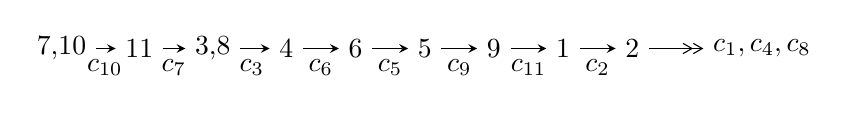
\begin{tikzpicture}[x=25pt, y=7pt]
	% node
	\node (A0) at (-1/8, 0) {7,10};
	\node (A1) at (1, 0) {11};
	\node (A2) at (33/16, 0) {3,8};
	\node (A3) at (25/8, 0) {4};
	\node (A4) at (33/8, 0) {6};
	\node (A5) at (41/8, 0) {5};
	\node (A6) at (49/8, 0) {9};
	\node (A7) at (57/8, 0) {1};
	\node (A8) at (65/8, 0) {2};
	\node (C1) at (1/2, -1) {$c_{10}$};
	\node (C2) at (3/2, -1) {$c_{7}$};
	\node (C3) at (21/8, -1) {$c_{3}$};
	\node (C4) at (29/8, -1) {$c_{6}$};
	\node (C5) at (37/8, -1) {$c_{5}$};
	\node (C6) at (45/8, -1) {$c_{9}$};
	\node (C7) at (53/8, -1) {$c_{11}$};
	\node (C8) at (61/8, -1) {$c_{2}$};
	\node (A9) at (10, 0) {$c_{1},c_{4},c_{8}$};

	% edge
	\draw[->,>=stealth]	
	(A0) edge (A1) (A1) edge (A2) (A2) edge (A3) (A3) edge (A4) (A4) edge (A5) (A5) edge (A6) (A6) edge (A7) (A7) edge (A8) ;
	\draw[->>,>={angle 60}]	
	(A8) edge (A9);
\end{tikzpicture} \\ 

\end{tabular} \\

\footnotetext{
The image of knot diagram is generated by the software ``\textbf{Draw programme}" developed by Andrew Bartholomew(\url{http://www.layer8.co.uk/maths/draw/index.htm\#Running-draw}), where we modified some parts for our purpose(\url{https://github.com/CATsTAILs/LinksPainter}).
}\phantom \\ \newline 
\centering \textbf{Ideals for irreducible components\footnotemark of $X_{\text{par}}$} 
 
\begin{align*}
I^u_{1}&=\langle 
-17 u^{50}+25 u^{49}+\cdots+2 b-13,\;15 u^{50}-24 u^{49}+\cdots+2 a+6,\;u^{51}-3 u^{50}+\cdots-3 u^2-1\rangle \\
I^u_{2}&=\langle 
- a u+b,\;a^2- a+1,\;u^2+u-1\rangle \\
\\
\end{align*}
\raggedright * 2 irreducible components of $\dim_{\mathbb{C}}=0$, with total 55 representations.\\
\footnotetext{All coefficients of polynomials are rational numbers. But the coefficients are sometimes approximated in decimal forms when there is not enough margin.}
\newpage
\renewcommand{\arraystretch}{1}
\centering \section*{I. $I^u_{1}= \langle -17 u^{50}+25 u^{49}+\cdots+2 b-13,\;15 u^{50}-24 u^{49}+\cdots+2 a+6,\;u^{51}-3 u^{50}+\cdots-3 u^2-1 \rangle$}
\flushleft \textbf{(i) Arc colorings}\\
\begin{tabular}{m{7pt} m{180pt} m{7pt} m{180pt} }
\flushright $a_{7}=$&$\begin{pmatrix}0\\u\end{pmatrix}$ \\
\flushright $a_{10}=$&$\begin{pmatrix}1\\0\end{pmatrix}$ \\
\flushright $a_{11}=$&$\begin{pmatrix}1\\- u^2\end{pmatrix}$ \\
\flushright $a_{3}=$&$\begin{pmatrix}-\frac{15}{2} u^{50}+12 u^{49}+\cdots-\frac{5}{2} u-3\\\frac{17}{2} u^{50}-\frac{25}{2} u^{49}+\cdots+2 u+\frac{13}{2}\end{pmatrix}$ \\
\flushright $a_{8}=$&$\begin{pmatrix}u\\- u^3+u\end{pmatrix}$ \\
\flushright $a_{4}=$&$\begin{pmatrix}-\frac{17}{2} u^{50}+13 u^{49}+\cdots-\frac{5}{2} u-3\\\frac{25}{2} u^{50}-\frac{33}{2} u^{49}+\cdots+3 u+\frac{17}{2}\end{pmatrix}$ \\
\flushright $a_{6}=$&$\begin{pmatrix}- u\\u\end{pmatrix}$ \\
\flushright $a_{5}=$&$\begin{pmatrix}-\frac{1}{2} u^{50}+u^{49}+\cdots+\frac{3}{2} u-1\\\frac{1}{2} u^{50}-\frac{1}{2} u^{49}+\cdots+2 u+\frac{1}{2}\end{pmatrix}$ \\
\flushright $a_{9}=$&$\begin{pmatrix}- u^2+1\\u^2\end{pmatrix}$ \\
\flushright $a_{1}=$&$\begin{pmatrix}- u^6+3 u^4-2 u^2+1\\u^6-2 u^4- u^2\end{pmatrix}$ \\
\flushright $a_{2}=$&$\begin{pmatrix}-8 u^{50}+\frac{25}{2} u^{49}+\cdots-\frac{7}{2} u-\frac{5}{2}\\11 u^{50}-15 u^{49}+\cdots+3 u+8\end{pmatrix}$\\ \flushright $a_{2}=$&$\begin{pmatrix}-8 u^{50}+\frac{25}{2} u^{49}+\cdots-\frac{7}{2} u-\frac{5}{2}\\11 u^{50}-15 u^{49}+\cdots+3 u+8\end{pmatrix}$\\&\end{tabular}
\flushleft \textbf{(ii) Obstruction class $= -1$}\\~\\
\flushleft \textbf{(iii) Cusp Shapes $= -\frac{5}{2} u^{50}+3 u^{49}+\cdots+\frac{1}{2} u^2-\frac{11}{2} u$}\\~\\
\newpage\renewcommand{\arraystretch}{1}
\flushleft \textbf{(iv) u-Polynomials at the component}\newline \\
\begin{tabular}{m{50pt}|m{274pt}}
Crossings & \hspace{64pt}u-Polynomials at each crossing \\
\hline $$\begin{aligned}c_{1},c_{4}\end{aligned}$$&$\begin{aligned}
&u^{51}+3 u^{50}+\cdots+4 u+1
\end{aligned}$\\
\hline $$\begin{aligned}c_{2}\end{aligned}$$&$\begin{aligned}
&u^{51}+25 u^{50}+\cdots-2 u-1
\end{aligned}$\\
\hline $$\begin{aligned}c_{3},c_{8}\end{aligned}$$&$\begin{aligned}
&u^{51}- u^{50}+\cdots+100 u^2-16
\end{aligned}$\\
\hline $$\begin{aligned}c_{5}\end{aligned}$$&$\begin{aligned}
&u^{51}-3 u^{50}+\cdots-488 u+241
\end{aligned}$\\
\hline $$\begin{aligned}c_{6},c_{7},c_{9}\\c_{10}\end{aligned}$$&$\begin{aligned}
&u^{51}-3 u^{50}+\cdots-3 u^2-1
\end{aligned}$\\
\hline $$\begin{aligned}c_{11}\end{aligned}$$&$\begin{aligned}
&u^{51}+13 u^{50}+\cdots+102 u-7
\end{aligned}$\\
\hline
\end{tabular}\\~\\
\newpage\renewcommand{\arraystretch}{1}
\flushleft \textbf{(v) Riley Polynomials at the component}\newline \\
\begin{tabular}{m{50pt}|m{274pt}}
Crossings & \hspace{64pt}Riley Polynomials at each crossing \\
\hline $$\begin{aligned}c_{1},c_{4}\end{aligned}$$&$\begin{aligned}
&y^{51}+25 y^{50}+\cdots-2 y-1
\end{aligned}$\\
\hline $$\begin{aligned}c_{2}\end{aligned}$$&$\begin{aligned}
&y^{51}+5 y^{50}+\cdots-42 y-1
\end{aligned}$\\
\hline $$\begin{aligned}c_{3},c_{8}\end{aligned}$$&$\begin{aligned}
&y^{51}-25 y^{50}+\cdots+3200 y-256
\end{aligned}$\\
\hline $$\begin{aligned}c_{5}\end{aligned}$$&$\begin{aligned}
&y^{51}-15 y^{50}+\cdots+378406 y-58081
\end{aligned}$\\
\hline $$\begin{aligned}c_{6},c_{7},c_{9}\\c_{10}\end{aligned}$$&$\begin{aligned}
&y^{51}-59 y^{50}+\cdots-6 y-1
\end{aligned}$\\
\hline $$\begin{aligned}c_{11}\end{aligned}$$&$\begin{aligned}
&y^{51}+y^{50}+\cdots+27134 y-49
\end{aligned}$\\
\hline
\end{tabular}\\~\\
\newpage\flushleft \textbf{(vi) Complex Volumes and Cusp Shapes}
$$\begin{array}{c|c|c}  
\text{Solutions to }I^u_{1}& \I (\text{vol} + \sqrt{-1}CS) & \text{Cusp shape}\\
 \hline 
\begin{aligned}
u &= \phantom{-}1.010040 + 0.185114 I \\
a &= \phantom{-}0.028727 + 0.217779 I \\
b &= \phantom{-}1.155140 + 0.071848 I\end{aligned}
 & -0.74107 - 3.69137 I & \phantom{-}3.00000 + 3.57636 I \\ \hline\begin{aligned}
u &= \phantom{-}1.010040 - 0.185114 I \\
a &= \phantom{-}0.028727 - 0.217779 I \\
b &= \phantom{-}1.155140 - 0.071848 I\end{aligned}
 & -0.74107 + 3.69137 I & \phantom{-}3.00000 - 3.57636 I \\ \hline\begin{aligned}
u &= -0.696278 + 0.562745 I \\
a &= -0.126496 - 0.100580 I \\
b &= -0.65483 - 1.57526 I\end{aligned}
 & -3.44622 - 10.79080 I & \phantom{-}1.49962 + 9.34961 I \\ \hline\begin{aligned}
u &= -0.696278 - 0.562745 I \\
a &= -0.126496 + 0.100580 I \\
b &= -0.65483 + 1.57526 I\end{aligned}
 & -3.44622 + 10.79080 I & \phantom{-}1.49962 - 9.34961 I \\ \hline\begin{aligned}
u &= -0.669411 + 0.527277 I \\
a &= -0.078362 + 0.148261 I \\
b &= \phantom{-}0.48562 + 1.39970 I\end{aligned}
 & -0.91928 - 5.72397 I & \phantom{-}4.37797 + 6.08222 I \\ \hline\begin{aligned}
u &= -0.669411 - 0.527277 I \\
a &= -0.078362 - 0.148261 I \\
b &= \phantom{-}0.48562 - 1.39970 I\end{aligned}
 & -0.91928 + 5.72397 I & \phantom{-}4.37797 - 6.08222 I \\ \hline\begin{aligned}
u &= -0.601097 + 0.571095 I \\
a &= \phantom{-}0.200819 + 0.207134 I \\
b &= -0.716384 - 1.036900 I\end{aligned}
 & -5.51696 - 2.60444 I & -1.87192 + 3.52202 I \\ \hline\begin{aligned}
u &= -0.601097 - 0.571095 I \\
a &= \phantom{-}0.200819 - 0.207134 I \\
b &= -0.716384 + 1.036900 I\end{aligned}
 & -5.51696 + 2.60444 I & -1.87192 - 3.52202 I \\ \hline\begin{aligned}
u &= \phantom{-}0.782212 + 0.168121 I \\
a &= \phantom{-}0.268689 - 0.110103 I \\
b &= -0.800842 - 0.378551 I\end{aligned}
 & \phantom{-}1.51394 + 0.22954 I & \phantom{-}7.32004 + 0.16659 I \\ \hline\begin{aligned}
u &= \phantom{-}0.782212 - 0.168121 I \\
a &= \phantom{-}0.268689 + 0.110103 I \\
b &= -0.800842 + 0.378551 I\end{aligned}
 & \phantom{-}1.51394 - 0.22954 I & \phantom{-}7.32004 - 0.16659 I\\
 \hline 
 \end{array}$$\newpage$$\begin{array}{c|c|c}  
\text{Solutions to }I^u_{1}& \I (\text{vol} + \sqrt{-1}CS) & \text{Cusp shape}\\
 \hline 
\begin{aligned}
u &= \phantom{-}0.579058 + 0.450651 I \\
a &= -1.037300 + 0.151216 I \\
b &= \phantom{-}0.36687 + 1.44155 I\end{aligned}
 & -0.67124 + 4.97036 I & \phantom{-}2.71900 - 7.31464 I \\ \hline\begin{aligned}
u &= \phantom{-}0.579058 - 0.450651 I \\
a &= -1.037300 - 0.151216 I \\
b &= \phantom{-}0.36687 - 1.44155 I\end{aligned}
 & -0.67124 - 4.97036 I & \phantom{-}2.71900 + 7.31464 I \\ \hline\begin{aligned}
u &= -0.343524 + 0.624420 I \\
a &= -0.976295 - 0.922559 I \\
b &= \phantom{-}0.269931 - 0.191977 I\end{aligned}
 & -6.27450 - 1.45252 I & -3.69386 + 3.06697 I \\ \hline\begin{aligned}
u &= -0.343524 - 0.624420 I \\
a &= -0.976295 + 0.922559 I \\
b &= \phantom{-}0.269931 + 0.191977 I\end{aligned}
 & -6.27450 + 1.45252 I & -3.69386 - 3.06697 I \\ \hline\begin{aligned}
u &= -0.599839 + 0.369476 I \\
a &= -0.798578 + 0.484702 I \\
b &= -0.125617 + 1.082760 I\end{aligned}
 & \phantom{-}1.18905 - 3.57721 I & \phantom{-}4.64362 + 8.91865 I \\ \hline\begin{aligned}
u &= -0.599839 - 0.369476 I \\
a &= -0.798578 - 0.484702 I \\
b &= -0.125617 - 1.082760 I\end{aligned}
 & \phantom{-}1.18905 + 3.57721 I & \phantom{-}4.64362 - 8.91865 I \\ \hline\begin{aligned}
u &= -0.228379 + 0.658723 I \\
a &= -1.28242 - 1.11756 I \\
b &= -0.201046 - 0.506980 I\end{aligned}
 & -4.82761 + 6.67077 I & -1.71165 - 4.27909 I \\ \hline\begin{aligned}
u &= -0.228379 - 0.658723 I \\
a &= -1.28242 + 1.11756 I \\
b &= -0.201046 + 0.506980 I\end{aligned}
 & -4.82761 - 6.67077 I & -1.71165 + 4.27909 I \\ \hline\begin{aligned}
u &= \phantom{-}0.614370 + 0.324141 I \\
a &= \phantom{-}0.701582 - 0.039747 I \\
b &= -0.491878 - 0.972906 I\end{aligned}
 & \phantom{-}1.41349 + 0.80124 I & \phantom{-}7.83477 - 2.87289 I \\ \hline\begin{aligned}
u &= \phantom{-}0.614370 - 0.324141 I \\
a &= \phantom{-}0.701582 + 0.039747 I \\
b &= -0.491878 + 0.972906 I\end{aligned}
 & \phantom{-}1.41349 - 0.80124 I & \phantom{-}7.83477 + 2.87289 I\\
 \hline 
 \end{array}$$\newpage$$\begin{array}{c|c|c}  
\text{Solutions to }I^u_{1}& \I (\text{vol} + \sqrt{-1}CS) & \text{Cusp shape}\\
 \hline 
\begin{aligned}
u &= -0.243226 + 0.591006 I \\
a &= \phantom{-}1.28551 + 0.93694 I \\
b &= \phantom{-}0.170934 + 0.215041 I\end{aligned}
 & -2.16539 + 1.90010 I & \phantom{-}1.028545 - 0.515555 I \\ \hline\begin{aligned}
u &= -0.243226 - 0.591006 I \\
a &= \phantom{-}1.28551 - 0.93694 I \\
b &= \phantom{-}0.170934 - 0.215041 I\end{aligned}
 & -2.16539 - 1.90010 I & \phantom{-}1.028545 + 0.515555 I \\ \hline\begin{aligned}
u &= \phantom{-}1.366540 + 0.105513 I \\
a &= \phantom{-}0.073383 - 0.327087 I \\
b &= \phantom{-}0.780564 + 0.143090 I\end{aligned}
 & -0.93634 + 4.10134 I & \phantom{-0.000000 } 0 \\ \hline\begin{aligned}
u &= \phantom{-}1.366540 - 0.105513 I \\
a &= \phantom{-}0.073383 + 0.327087 I \\
b &= \phantom{-}0.780564 - 0.143090 I\end{aligned}
 & -0.93634 - 4.10134 I & \phantom{-0.000000 } 0 \\ \hline\begin{aligned}
u &= \phantom{-}1.40634\phantom{ +0.000000I} \\
a &= \phantom{-}0.303169\phantom{ +0.000000I} \\
b &= -1.14879\phantom{ +0.000000I}\end{aligned}
 & \phantom{-}2.53581\phantom{ +0.000000I} & \phantom{-0.000000 } 0 \\ \hline\begin{aligned}
u &= -0.511782 + 0.272136 I \\
a &= \phantom{-}1.43457 - 0.46586 I \\
b &= \phantom{-}0.446013 - 0.822688 I\end{aligned}
 & \phantom{-}0.64233 + 1.35638 I & \phantom{-}0.89935 + 4.08945 I \\ \hline\begin{aligned}
u &= -0.511782 - 0.272136 I \\
a &= \phantom{-}1.43457 + 0.46586 I \\
b &= \phantom{-}0.446013 + 0.822688 I\end{aligned}
 & \phantom{-}0.64233 - 1.35638 I & \phantom{-}0.89935 - 4.08945 I \\ \hline\begin{aligned}
u &= \phantom{-}0.359561 + 0.428490 I \\
a &= -1.281080 - 0.420225 I \\
b &= -0.329117 + 1.066960 I\end{aligned}
 & -1.31778 - 1.81267 I & \phantom{-}0.238643 - 0.120411 I \\ \hline\begin{aligned}
u &= \phantom{-}0.359561 - 0.428490 I \\
a &= -1.281080 + 0.420225 I \\
b &= -0.329117 - 1.066960 I\end{aligned}
 & -1.31778 + 1.81267 I & \phantom{-}0.238643 + 0.120411 I \\ \hline\begin{aligned}
u &= -1.51828 + 0.07351 I \\
a &= \phantom{-}0.37450 - 1.82930 I \\
b &= \phantom{-}0.11043 + 1.78445 I\end{aligned}
 & \phantom{-}4.98533 + 0.33539 I & \phantom{-0.000000 } 0\\
 \hline 
 \end{array}$$\newpage$$\begin{array}{c|c|c}  
\text{Solutions to }I^u_{1}& \I (\text{vol} + \sqrt{-1}CS) & \text{Cusp shape}\\
 \hline 
\begin{aligned}
u &= -1.51828 - 0.07351 I \\
a &= \phantom{-}0.37450 + 1.82930 I \\
b &= \phantom{-}0.11043 - 1.78445 I\end{aligned}
 & \phantom{-}4.98533 - 0.33539 I & \phantom{-0.000000 } 0 \\ \hline\begin{aligned}
u &= \phantom{-}1.56233 + 0.08226 I \\
a &= \phantom{-}1.12351 + 1.94512 I \\
b &= -1.69642 - 2.80365 I\end{aligned}
 & \phantom{-}7.78597 - 0.04605 I & \phantom{-0.000000 } 0 \\ \hline\begin{aligned}
u &= \phantom{-}1.56233 - 0.08226 I \\
a &= \phantom{-}1.12351 - 1.94512 I \\
b &= -1.69642 + 2.80365 I\end{aligned}
 & \phantom{-}7.78597 + 0.04605 I & \phantom{-0.000000 } 0 \\ \hline\begin{aligned}
u &= \phantom{-}1.56086 + 0.16665 I \\
a &= -0.23171 + 1.99295 I \\
b &= \phantom{-}0.61349 - 2.25582 I\end{aligned}
 & \phantom{-}1.69351 + 5.28998 I & \phantom{-0.000000 } 0 \\ \hline\begin{aligned}
u &= \phantom{-}1.56086 - 0.16665 I \\
a &= -0.23171 - 1.99295 I \\
b &= \phantom{-}0.61349 + 2.25582 I\end{aligned}
 & \phantom{-}1.69351 - 5.28998 I & \phantom{-0.000000 } 0 \\ \hline\begin{aligned}
u &= -1.56649 + 0.12512 I \\
a &= \phantom{-}0.81106 - 1.94624 I \\
b &= -0.02960 + 2.45788 I\end{aligned}
 & \phantom{-}6.58151 - 7.03980 I & \phantom{-0.000000 } 0 \\ \hline\begin{aligned}
u &= -1.56649 - 0.12512 I \\
a &= \phantom{-}0.81106 + 1.94624 I \\
b &= -0.02960 - 2.45788 I\end{aligned}
 & \phantom{-}6.58151 + 7.03980 I & \phantom{-0.000000 } 0 \\ \hline\begin{aligned}
u &= \phantom{-}1.57533 + 0.10647 I \\
a &= -0.67114 - 2.26632 I \\
b &= \phantom{-}0.83041 + 3.20187 I\end{aligned}
 & \phantom{-}8.59223 + 5.32247 I & \phantom{-0.000000 } 0 \\ \hline\begin{aligned}
u &= \phantom{-}1.57533 - 0.10647 I \\
a &= -0.67114 + 2.26632 I \\
b &= \phantom{-}0.83041 - 3.20187 I\end{aligned}
 & \phantom{-}8.59223 - 5.32247 I & \phantom{-0.000000 } 0 \\ \hline\begin{aligned}
u &= -1.57717 + 0.09542 I \\
a &= -0.78995 + 1.70101 I \\
b &= \phantom{-}0.32037 - 2.17607 I\end{aligned}
 & \phantom{-}8.87289 - 2.35791 I & \phantom{-0.000000 } 0\\
 \hline 
 \end{array}$$\newpage$$\begin{array}{c|c|c}  
\text{Solutions to }I^u_{1}& \I (\text{vol} + \sqrt{-1}CS) & \text{Cusp shape}\\
 \hline 
\begin{aligned}
u &= -1.57717 - 0.09542 I \\
a &= -0.78995 - 1.70101 I \\
b &= \phantom{-}0.32037 + 2.17607 I\end{aligned}
 & \phantom{-}8.87289 + 2.35791 I & \phantom{-0.000000 } 0 \\ \hline\begin{aligned}
u &= \phantom{-}1.59320 + 0.15654 I \\
a &= \phantom{-}0.17669 - 2.45152 I \\
b &= -0.80910 + 3.14034 I\end{aligned}
 & \phantom{-}6.71685 + 8.26103 I & \phantom{-0.000000 } 0 \\ \hline\begin{aligned}
u &= \phantom{-}1.59320 - 0.15654 I \\
a &= \phantom{-}0.17669 + 2.45152 I \\
b &= -0.80910 - 3.14034 I\end{aligned}
 & \phantom{-}6.71685 - 8.26103 I & \phantom{-0.000000 } 0 \\ \hline\begin{aligned}
u &= \phantom{-}1.60213 + 0.17042 I \\
a &= -0.39966 + 2.52070 I \\
b &= \phantom{-}1.29169 - 3.13581 I\end{aligned}
 & \phantom{-}4.3011 + 13.5338 I & \phantom{-0.000000 } 0 \\ \hline\begin{aligned}
u &= \phantom{-}1.60213 - 0.17042 I \\
a &= -0.39966 - 2.52070 I \\
b &= \phantom{-}1.29169 + 3.13581 I\end{aligned}
 & \phantom{-}4.3011 - 13.5338 I & \phantom{-0.000000 } 0 \\ \hline\begin{aligned}
u &= -1.62797 + 0.05185 I \\
a &= -1.03715 + 1.00610 I \\
b &= \phantom{-}1.17135 - 1.51034 I\end{aligned}
 & \phantom{-}9.84168 - 1.12988 I & \phantom{-0.000000 } 0 \\ \hline\begin{aligned}
u &= -1.62797 - 0.05185 I \\
a &= -1.03715 - 1.00610 I \\
b &= \phantom{-}1.17135 + 1.51034 I\end{aligned}
 & \phantom{-}9.84168 + 1.12988 I & \phantom{-0.000000 } 0 \\ \hline\begin{aligned}
u &= -1.66201 + 0.03190 I \\
a &= \phantom{-}1.44313 - 0.54681 I \\
b &= -2.00594 + 0.95171 I\end{aligned}
 & \phantom{-}8.41785 + 2.99724 I & \phantom{-0.000000 } 0 \\ \hline\begin{aligned}
u &= -1.66201 - 0.03190 I \\
a &= \phantom{-}1.44313 + 0.54681 I \\
b &= -2.00594 - 0.95171 I\end{aligned}
 & \phantom{-}8.41785 - 2.99724 I & \phantom{-0.000000 } 0 \\ \hline\begin{aligned}
u &= \phantom{-}0.036663 + 0.311170 I \\
a &= \phantom{-}1.63637 + 1.04446 I \\
b &= \phantom{-}0.422361 - 0.375155 I\end{aligned}
 & -0.118620 + 1.395530 I & -0.02533 - 5.05336 I\\
 \hline 
 \end{array}$$\newpage$$\begin{array}{c|c|c}  
\text{Solutions to }I^u_{1}& \I (\text{vol} + \sqrt{-1}CS) & \text{Cusp shape}\\
 \hline 
\begin{aligned}
u &= \phantom{-}0.036663 - 0.311170 I \\
a &= \phantom{-}1.63637 - 1.04446 I \\
b &= \phantom{-}0.422361 + 0.375155 I\end{aligned}
 & -0.118620 - 1.395530 I & -0.02533 + 5.05336 I\\
 \hline 
 \end{array}$$\newpage\newpage\renewcommand{\arraystretch}{1}
\centering \section*{II. $I^u_{2}= \langle - a u+b,\;a^2- a+1,\;u^2+u-1 \rangle$}
\flushleft \textbf{(i) Arc colorings}\\
\begin{tabular}{m{7pt} m{180pt} m{7pt} m{180pt} }
\flushright $a_{7}=$&$\begin{pmatrix}0\\u\end{pmatrix}$ \\
\flushright $a_{10}=$&$\begin{pmatrix}1\\0\end{pmatrix}$ \\
\flushright $a_{11}=$&$\begin{pmatrix}1\\u-1\end{pmatrix}$ \\
\flushright $a_{3}=$&$\begin{pmatrix}a\\a u\end{pmatrix}$ \\
\flushright $a_{8}=$&$\begin{pmatrix}u\\- u+1\end{pmatrix}$ \\
\flushright $a_{4}=$&$\begin{pmatrix}a\\a u\end{pmatrix}$ \\
\flushright $a_{6}=$&$\begin{pmatrix}- u\\u\end{pmatrix}$ \\
\flushright $a_{5}=$&$\begin{pmatrix}a- u-1\\a u\end{pmatrix}$ \\
\flushright $a_{9}=$&$\begin{pmatrix}u\\- u+1\end{pmatrix}$ \\
\flushright $a_{1}=$&$\begin{pmatrix}u\\- u\end{pmatrix}$ \\
\flushright $a_{2}=$&$\begin{pmatrix}a u+a\\0\end{pmatrix}$\\ \flushright $a_{2}=$&$\begin{pmatrix}a u+a\\0\end{pmatrix}$\\&\end{tabular}
\flushleft \textbf{(ii) Obstruction class $= 1$}\\~\\
\flushleft \textbf{(iii) Cusp Shapes $= 2 a u+5 a- u+4$}\\~\\
\newpage\renewcommand{\arraystretch}{1}
\flushleft \textbf{(iv) u-Polynomials at the component}\newline \\
\begin{tabular}{m{50pt}|m{274pt}}
Crossings & \hspace{64pt}u-Polynomials at each crossing \\
\hline $$\begin{aligned}c_{1},c_{2},c_{5}\end{aligned}$$&$\begin{aligned}
&(u^2+u+1)^2
\end{aligned}$\\
\hline $$\begin{aligned}c_{3},c_{8}\end{aligned}$$&$\begin{aligned}
&u^4
\end{aligned}$\\
\hline $$\begin{aligned}c_{4}\end{aligned}$$&$\begin{aligned}
&(u^2- u+1)^2
\end{aligned}$\\
\hline $$\begin{aligned}c_{6},c_{7}\end{aligned}$$&$\begin{aligned}
&(u^2- u-1)^2
\end{aligned}$\\
\hline $$\begin{aligned}c_{9},c_{10},c_{11}\end{aligned}$$&$\begin{aligned}
&(u^2+u-1)^2
\end{aligned}$\\
\hline
\end{tabular}\\~\\
\newpage\renewcommand{\arraystretch}{1}
\flushleft \textbf{(v) Riley Polynomials at the component}\newline \\
\begin{tabular}{m{50pt}|m{274pt}}
Crossings & \hspace{64pt}Riley Polynomials at each crossing \\
\hline $$\begin{aligned}c_{1},c_{2},c_{4}\\c_{5}\end{aligned}$$&$\begin{aligned}
&(y^2+y+1)^2
\end{aligned}$\\
\hline $$\begin{aligned}c_{3},c_{8}\end{aligned}$$&$\begin{aligned}
&y^4
\end{aligned}$\\
\hline $$\begin{aligned}c_{6},c_{7},c_{9}\\c_{10},c_{11}\end{aligned}$$&$\begin{aligned}
&(y^2-3 y+1)^2
\end{aligned}$\\
\hline
\end{tabular}\\~\\
\newpage\flushleft \textbf{(vi) Complex Volumes and Cusp Shapes}
$$\begin{array}{c|c|c}  
\text{Solutions to }I^u_{2}& \I (\text{vol} + \sqrt{-1}CS) & \text{Cusp shape}\\
 \hline 
\begin{aligned}
u &= \phantom{-}0.618034\phantom{ +0.000000I} \\
a &= \phantom{-}0.500000 + 0.866025 I \\
b &= \phantom{-}0.309017 + 0.535233 I\end{aligned}
 & \phantom{-}0.98696 - 2.02988 I & \phantom{-}6.50000 + 5.40059 I \\ \hline\begin{aligned}
u &= \phantom{-}0.618034\phantom{ +0.000000I} \\
a &= \phantom{-}0.500000 - 0.866025 I \\
b &= \phantom{-}0.309017 - 0.535233 I\end{aligned}
 & \phantom{-}0.98696 + 2.02988 I & \phantom{-}6.50000 - 5.40059 I \\ \hline\begin{aligned}
u &= -1.61803\phantom{ +0.000000I} \\
a &= \phantom{-}0.500000 + 0.866025 I \\
b &= -0.80902 - 1.40126 I\end{aligned}
 & \phantom{-}8.88264 - 2.02988 I & \phantom{-}6.50000 + 1.52761 I \\ \hline\begin{aligned}
u &= -1.61803\phantom{ +0.000000I} \\
a &= \phantom{-}0.500000 - 0.866025 I \\
b &= -0.80902 + 1.40126 I\end{aligned}
 & \phantom{-}8.88264 + 2.02988 I & \phantom{-}6.50000 - 1.52761 I\\
 \hline 
 \end{array}$$\newpage
\newpage\renewcommand{\arraystretch}{1}
\centering \section*{ III. u-Polynomials}
\begin{tabular}{m{50pt}|m{274pt}}
Crossings & \hspace{64pt}u-Polynomials at each crossing \\
\hline $$\begin{aligned}c_{1}\end{aligned}$$&$\begin{aligned}
&((u^2+u+1)^2)(u^{51}+3 u^{50}+\cdots+4 u+1)
\end{aligned}$\\
\hline $$\begin{aligned}c_{2}\end{aligned}$$&$\begin{aligned}
&((u^2+u+1)^2)(u^{51}+25 u^{50}+\cdots-2 u-1)
\end{aligned}$\\
\hline $$\begin{aligned}c_{3},c_{8}\end{aligned}$$&$\begin{aligned}
&u^4(u^{51}- u^{50}+\cdots+100 u^2-16)
\end{aligned}$\\
\hline $$\begin{aligned}c_{4}\end{aligned}$$&$\begin{aligned}
&((u^2- u+1)^2)(u^{51}+3 u^{50}+\cdots+4 u+1)
\end{aligned}$\\
\hline $$\begin{aligned}c_{5}\end{aligned}$$&$\begin{aligned}
&((u^2+u+1)^2)(u^{51}-3 u^{50}+\cdots-488 u+241)
\end{aligned}$\\
\hline $$\begin{aligned}c_{6},c_{7}\end{aligned}$$&$\begin{aligned}
&((u^2- u-1)^2)(u^{51}-3 u^{50}+\cdots-3 u^2-1)
\end{aligned}$\\
\hline $$\begin{aligned}c_{9},c_{10}\end{aligned}$$&$\begin{aligned}
&((u^2+u-1)^2)(u^{51}-3 u^{50}+\cdots-3 u^2-1)
\end{aligned}$\\
\hline $$\begin{aligned}c_{11}\end{aligned}$$&$\begin{aligned}
&((u^2+u-1)^2)(u^{51}+13 u^{50}+\cdots+102 u-7)
\end{aligned}$\\
\hline
\end{tabular}\newpage\renewcommand{\arraystretch}{1}
\centering \section*{ IV. Riley Polynomials}
\begin{tabular}{m{50pt}|m{274pt}}
Crossings & \hspace{64pt}Riley Polynomials at each crossing \\
\hline $$\begin{aligned}c_{1},c_{4}\end{aligned}$$&$\begin{aligned}
&((y^2+y+1)^2)(y^{51}+25 y^{50}+\cdots-2 y-1)
\end{aligned}$\\
\hline $$\begin{aligned}c_{2}\end{aligned}$$&$\begin{aligned}
&((y^2+y+1)^2)(y^{51}+5 y^{50}+\cdots-42 y-1)
\end{aligned}$\\
\hline $$\begin{aligned}c_{3},c_{8}\end{aligned}$$&$\begin{aligned}
&y^4(y^{51}-25 y^{50}+\cdots+3200 y-256)
\end{aligned}$\\
\hline $$\begin{aligned}c_{5}\end{aligned}$$&$\begin{aligned}
&((y^2+y+1)^2)(y^{51}-15 y^{50}+\cdots+378406 y-58081)
\end{aligned}$\\
\hline $$\begin{aligned}c_{6},c_{7},c_{9}\\c_{10}\end{aligned}$$&$\begin{aligned}
&((y^2-3 y+1)^2)(y^{51}-59 y^{50}+\cdots-6 y-1)
\end{aligned}$\\
\hline $$\begin{aligned}c_{11}\end{aligned}$$&$\begin{aligned}
&((y^2-3 y+1)^2)(y^{51}+y^{50}+\cdots+27134 y-49)
\end{aligned}$\\
\hline
\end{tabular}
\vskip 2pc
\end{document}